% Intended LaTeX compiler: pdflatex
\documentclass[10pt,a4paper,UTF8]{article}
\usepackage{zclorg}
\usepackage{tikztheorem}
\author{zcl.space}
\date{}
\title{优化多变量无约束函数利器:fminunc}
\hypersetup{
 pdfauthor={zcl.space},
 pdftitle={优化多变量无约束函数利器:fminunc},
 pdfkeywords={matlab optimization},
 pdfsubject={使用 \texttt{fminunc} 优化无约束多变量函数},
 pdfcreator={Emacs 25.0.50.1 (Org mode 9.1.2)},
 pdflang={English}}
\begin{document}

\maketitle
\tableofcontents
\titlepic{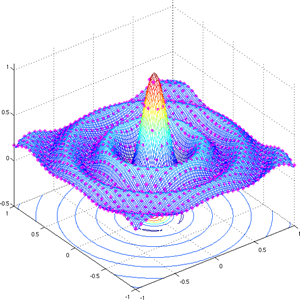
\includegraphics[scale=0.25]{../../img/sinc.PNG}}

\section{fminunc}
\label{sec:org8e95a76}


matlab提供了一个优化多变量无约束目标函数的利器:fminunc。

其实现的功能是:
\begin{equation}
\label{eq:1}
\underset{x}{\min}f(x)
\end{equation}

\section{应用1: \texttt{x = fminunc(fun,x0)}}
\label{sec:orgd12babd}


最简单的应用是:
\lstset{language=matlab,label= ,caption= ,captionpos=b,numbers=none}
\begin{lstlisting}
x = fminunc(fun,x0)
\end{lstlisting}

其中 \texttt{x = fminunc(fun,x0)} 提供了一个起始点\(x_{0}\),供 \texttt{fminunc} 使用。 \texttt{fminunc} 试图为目标函数找到局部最小解。

举个例子,假设要寻找函数\(f(x) = 3x_{1}^{2} + 2x_{1}x_{2}+ x_{2}^{2} -4x_{1} +5x_{2}\)的最小值。我们首先为这个函数提供一个匿名函数句柄:
\lstset{language=matlab,label= ,caption= ,captionpos=b,numbers=none}
\begin{lstlisting}
fun = @(x)3*x(1)^2 + 2*x(1)*x(2) + x(2)^2 - 4*x(1) + 5*x(2);
\end{lstlisting}
调用 \texttt{fminunc} :
\lstset{language=matlab,label= ,caption= ,captionpos=b,numbers=none}
\begin{lstlisting}
x0 =[1,1];
[x,fval] = fminunc(fun,x0);
\end{lstlisting}
经过若干次迭代后, \texttt{x} 返回最小值的位置, \texttt{fval} 返回目标函数在这个位置的最小值。
\begin{verbatim}
x,fval

x =

    2.2500   -4.7500


fval =

  -16.3750
\end{verbatim}
\section{应用2 : \texttt{x = fminunc(fun,x0,options)}}
\label{sec:org8d3f3ec}


当提供梯度结果的时候, \texttt{fmiunc} 的计算结果会大大加快。比如对于多变量Rosenbrock函数:
\begin{equation}
\label{eq:2}
f(x) = 100(x_{1} - x_{1}^{2})^{2} + (1-x_{1})^{2}
\end{equation}

其梯度为:
\begin{equation}
\label{eq:3}
\partial f(x) =
\begin{bmatrix}
-400(x_{1} - x_{1}^{2})x_{1} - 2(1-x_{1}) \\
200(x_{2} - x_{1}^{2})
\end{bmatrix}
\end{equation}

matlab 代码为:
\lstset{language=matlab,label= ,caption= ,captionpos=b,numbers=none}
\begin{lstlisting}
function [f,g] = rosenbrockwithgrad(x)
% Calculate objective f
f = 100*(x(2) - x(1)^2)^2 + (1-x(1))^2;

if nargout > 1 % gradient required
    g = [-400*(x(2)-x(1)^2)*x(1)-2*(1-x(1));
        200*(x(2)-x(1)^2)];
end
\end{lstlisting}

为这个目标函数的梯度提供一些参数:
\lstset{language=matlab,label= ,caption= ,captionpos=b,numbers=none}
\begin{lstlisting}
options = optimoptions('fminunc','Algorithm','trust-region','SpecifyObjectiveGradient',true);
\end{lstlisting}

设定初始值为 \([-1,2]\),然后调用 \texttt{fminunc}
\lstset{language=matlab,label= ,caption= ,captionpos=b,numbers=none}
\begin{lstlisting}
x0 = [-1,2];
fun = @rosenbrockwithgrad;
x = fminunc(fun,x0,options)
\end{lstlisting}
当梯度的值小于预先设定的最小值时,优化过程结束,程序返回:
\lstset{language=matlab,label= ,caption= ,captionpos=b,numbers=none}
\begin{lstlisting}
x =
  1.0000 1.0000
\end{lstlisting}
\section{应用3: \texttt{x = fminunc(problem)}}
\label{sec:org0fc90b3}


对于应用2 ,我们可以用更加结构化的方式来描述。首先还是针对Rosenbrock函数:

\begin{equation}
\label{eq:30}
f(x) = 100(x_{1} - x_{1}^{2})^{2} + (1-x_{1})^{2}
\end{equation}

其梯度为:
\begin{equation}
\label{eq:4}
\partial f(x) =
\begin{bmatrix}
-400(x_{1} - x_{1}^{2})x_{1} - 2(1-x_{1}) \\
200(x_{2} - x_{1}^{2})
\end{bmatrix}
\end{equation}

matlab代码跟之前一样:
\lstset{language=matlab,label= ,caption= ,captionpos=b,numbers=none}
\begin{lstlisting}
function [f,g] = rosenbrockwithgrad(x)
% Calculate objective f
f = 100*(x(2) - x(1)^2)^2 + (1-x(1))^2;

if nargout > 1 % gradient required
    g = [-400*(x(2)-x(1)^2)*x(1)-2*(1-x(1));
        200*(x(2)-x(1)^2)];
end
\end{lstlisting}

为目标函数梯度设定参数:
\lstset{language=matlab,label= ,caption= ,captionpos=b,numbers=none}
\begin{lstlisting}
options = optimoptions('fminunc','Algorithm','trust-region','SpecifyObjectiveGradient',true);
\end{lstlisting}

为所有的参数创建一个结构体:
\lstset{language=matlab,label= ,caption= ,captionpos=b,numbers=none}
\begin{lstlisting}
problem.options = options;
problem.x0 = [-1,2];
problem.objective = @rosenbrockwithgrad;
problem.solver = 'fminunc';
\end{lstlisting}

然后调用 \texttt{fminunc} :
\lstset{language=matlab,label= ,caption= ,captionpos=b,numbers=none}
\begin{lstlisting}
x = fminunc(problem)
\end{lstlisting}
\section{应用4: \texttt{[x,fval] = fminunc(fun,x0)}}
\label{sec:org6aad9b0}


\texttt{fminunc} 函数不仅可以找到最小值的位置,也可以返回最小值。只要对其添加第二个输出,就是局部最小值。

比如目标函数是:
\begin{equation}
\label{eq:5}
f(x) = x(1)e^{-||x||_{2}^{2}} + ||x||_{2}^{2}/20
\end{equation}
其MATLAB代码为:
\lstset{language=matlab,label= ,caption= ,captionpos=b,numbers=none}
\begin{lstlisting}
fun = @(x)x(1)*exp(-(x(1)^2 + x(2)^2)) + (x(1)^2 + x(2)^2)/20;
\end{lstlisting}
设定初始值,并调用 \texttt{fminunc} :
\lstset{language=matlab,label= ,caption= ,captionpos=b,numbers=none}
\begin{lstlisting}
x0 = [1,2];
[x,fval] = fminunc(fun,x0)
\end{lstlisting}
迭代结束后,返回:
\begin{verbatim}
x =

   -0.6691    0.0000

fval =

   -0.4052
\end{verbatim}
\section{总结}
\label{sec:orge2d8efa}


matlab已经把优化过程封装为一个函数了。我们要做的就是对问题建模,输出问题的数学模型,然后调用优化函数。

\texttt{fminunc} 的 \texttt{options} 选项还提供了更多的选择,比如是否显示迭代过程,采用的优化算法等等等等,这些可以通过查阅matlab的帮助文档悉知。
\end{document}
